\section{Appendix}

\begin{frame}[t]{Reale Bauteile modellieren mit einem subcircuit} 
    
    \begin{spacing}{0.9} \begin{tiny}
      \begin{table}[h!]
        \begin{tabular}{p{5cm} p{5cm}}
            \begin{minipage}{0.5\textwidth}
                Hier findet ihr eine Übersicht wie man ein reales Bauteil im Internet findet,
                den subcircuit einbindet und ein Modellfile dazu erzeugt. Diese Dateien sind Übernahmen
                aus dem alten Skript CAE Labor von Franz Smagacz-Allramseder. \newline

                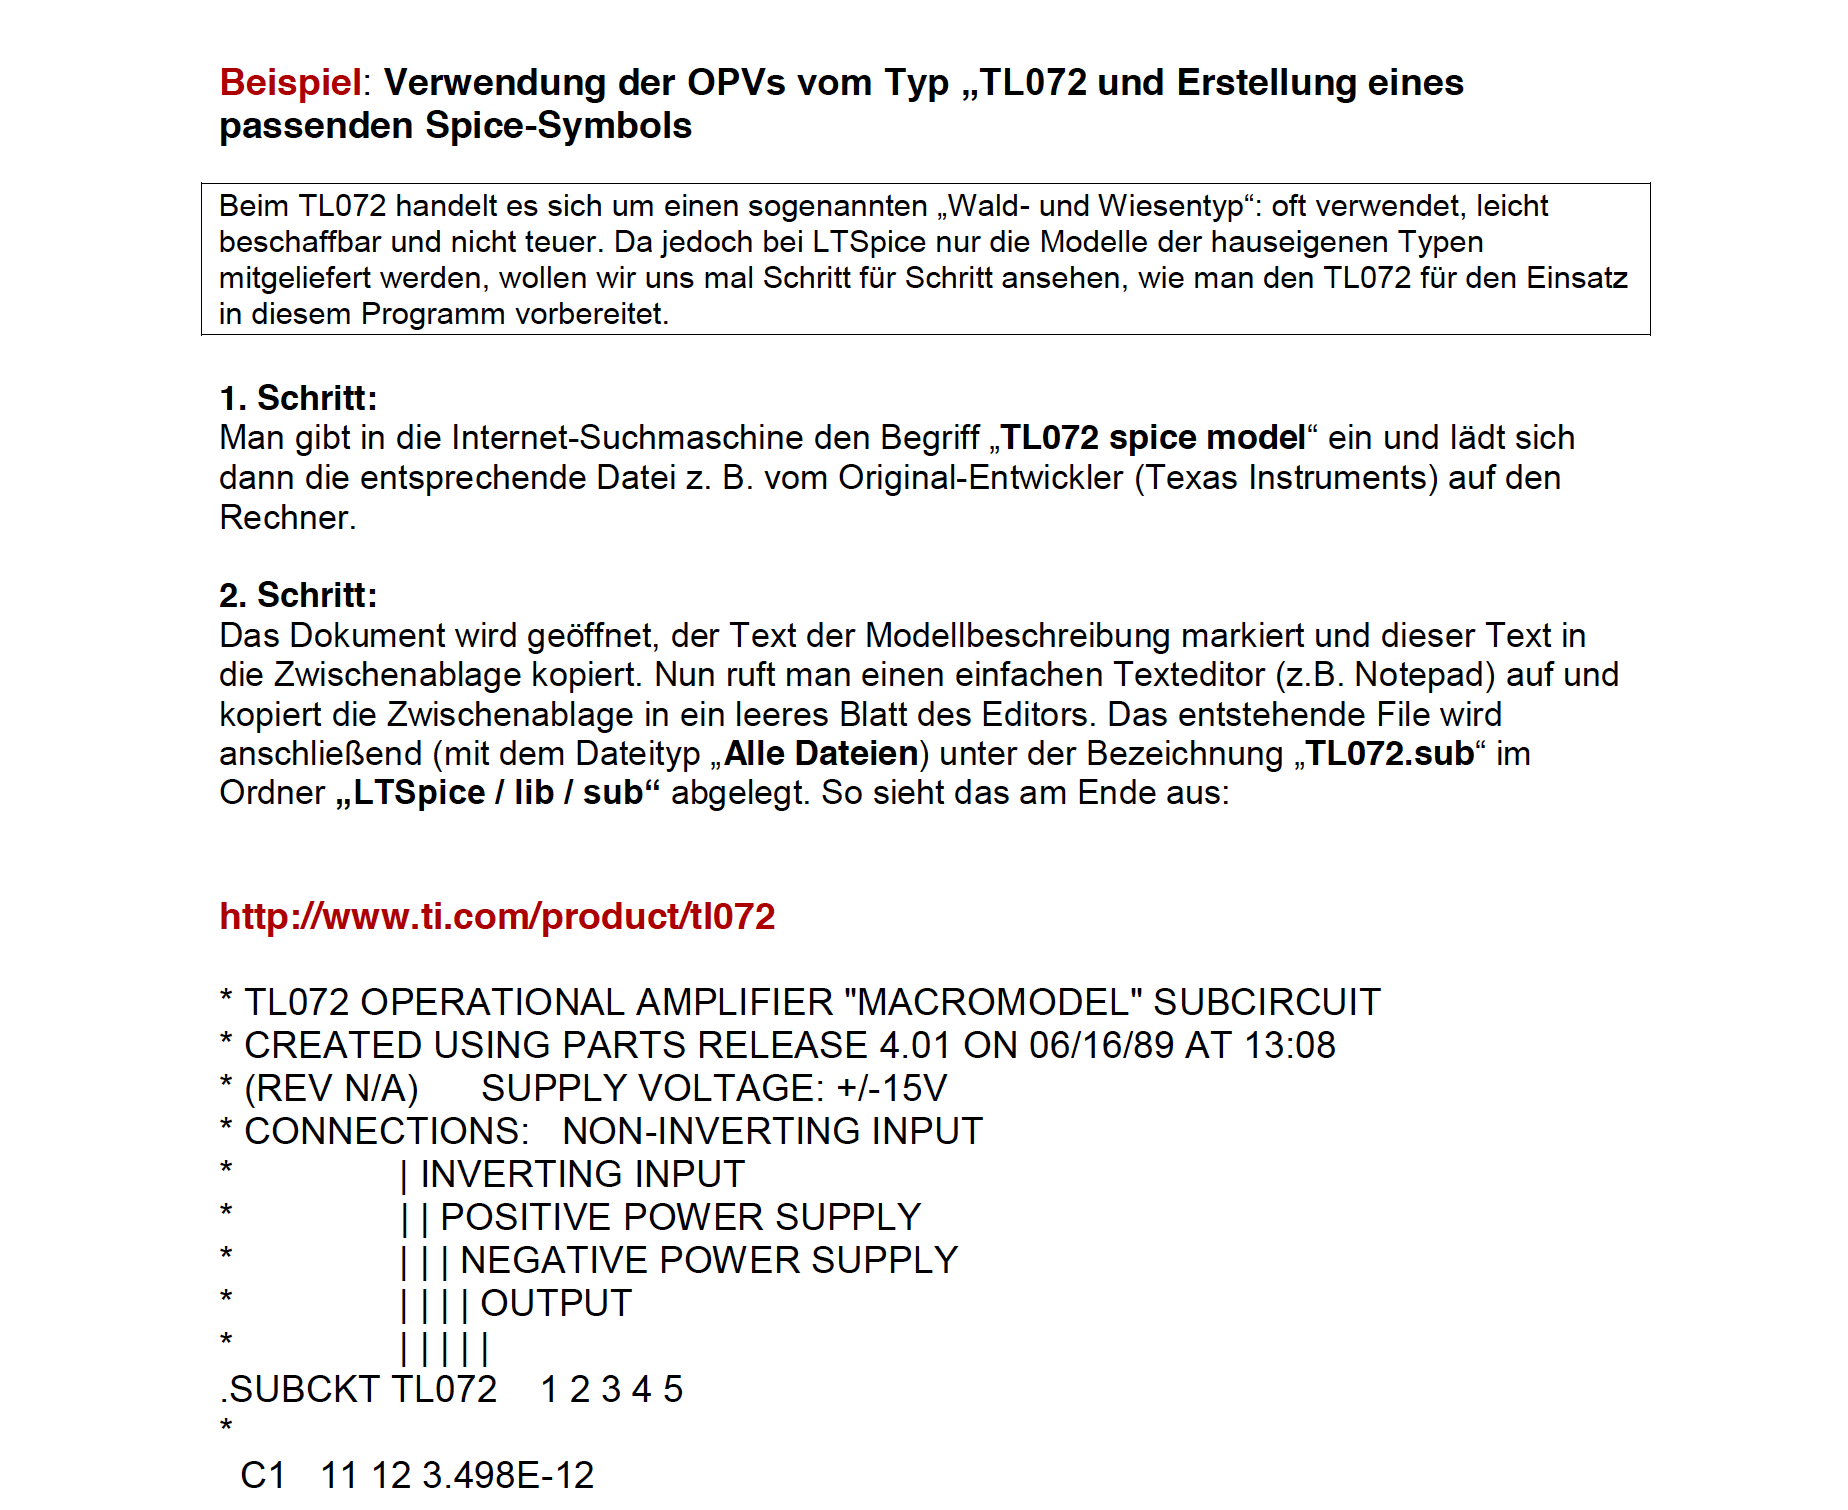
\includegraphics[width=\linewidth]{pictures/legacy/tl072_1.png}
            \end{minipage} 
            &
            \begin{minipage}{0.5\textwidth}
                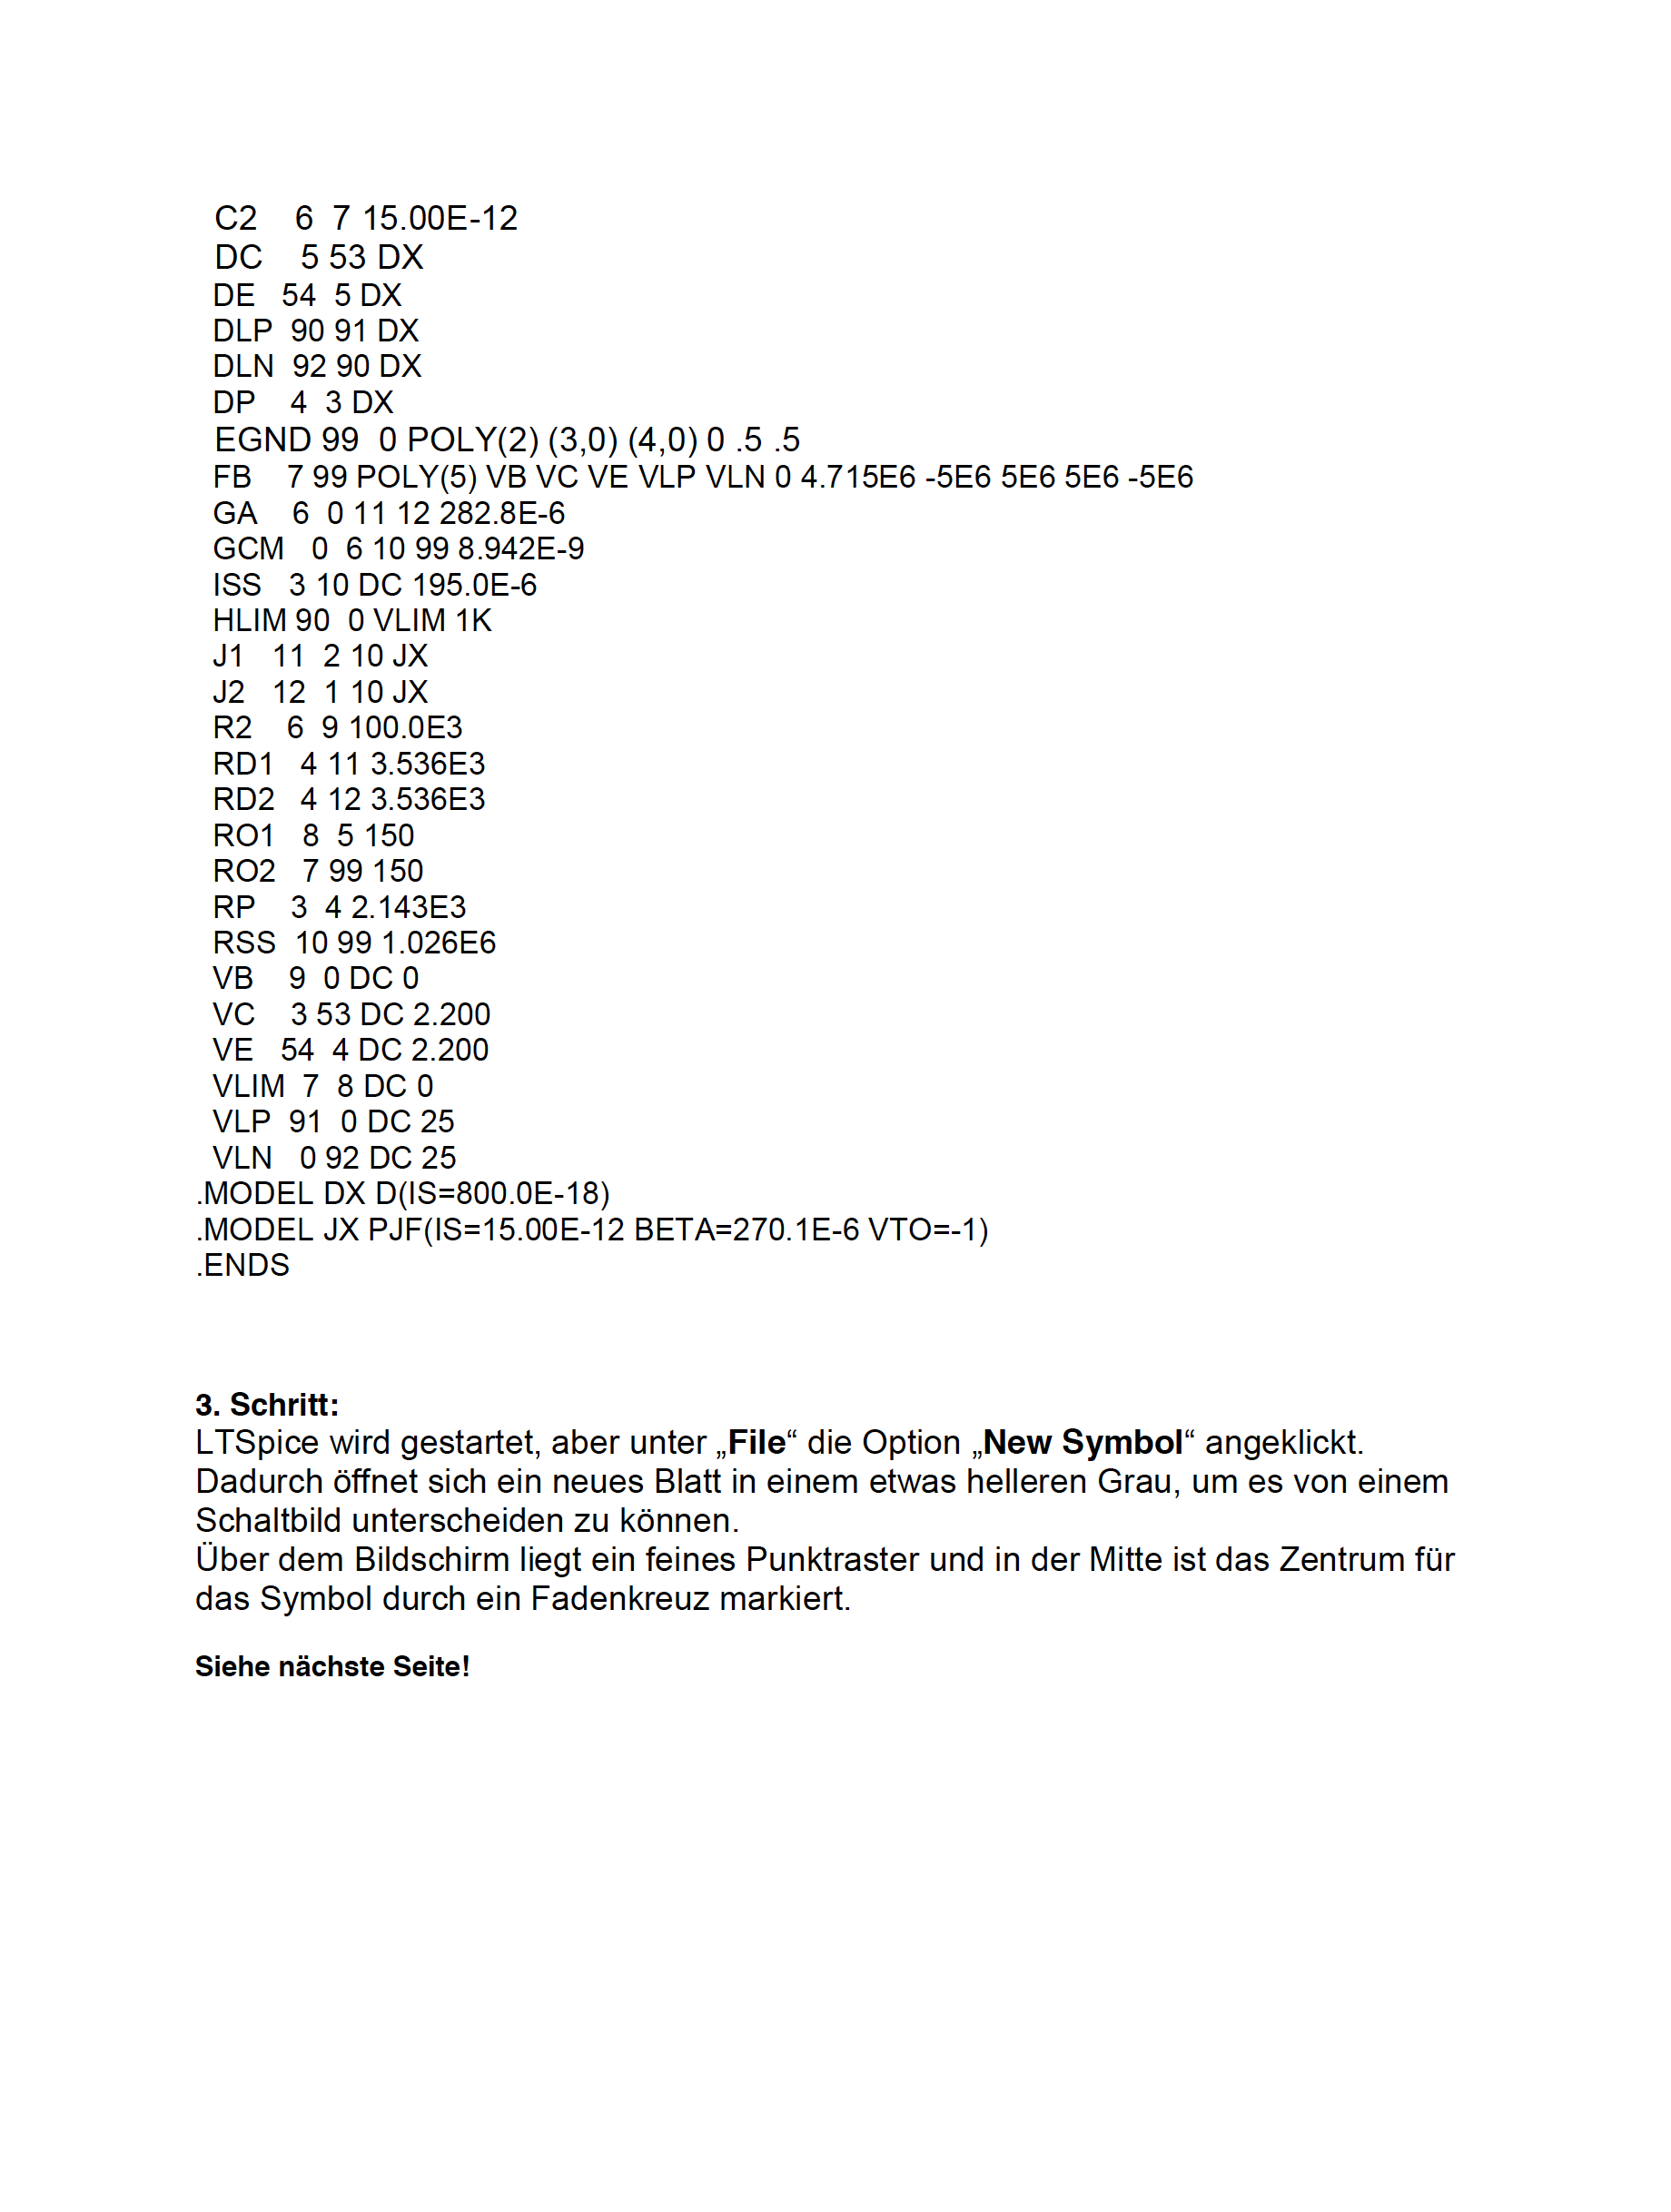
\includegraphics[width=\linewidth]{pictures/legacy/tl072_2.png}
            \end{minipage} 
      \end{tabular}
    \end{table}
    \end{tiny} \end{spacing}
\end{frame}

\begin{frame}[t]{Reale Bauteile modellieren mit einem subcircuit} 
    
    \begin{spacing}{0.9} \begin{tiny}
      \begin{table}[h!]
        \begin{tabular}{p{5cm} p{5cm}}
            \begin{minipage}{0.5\textwidth}                
                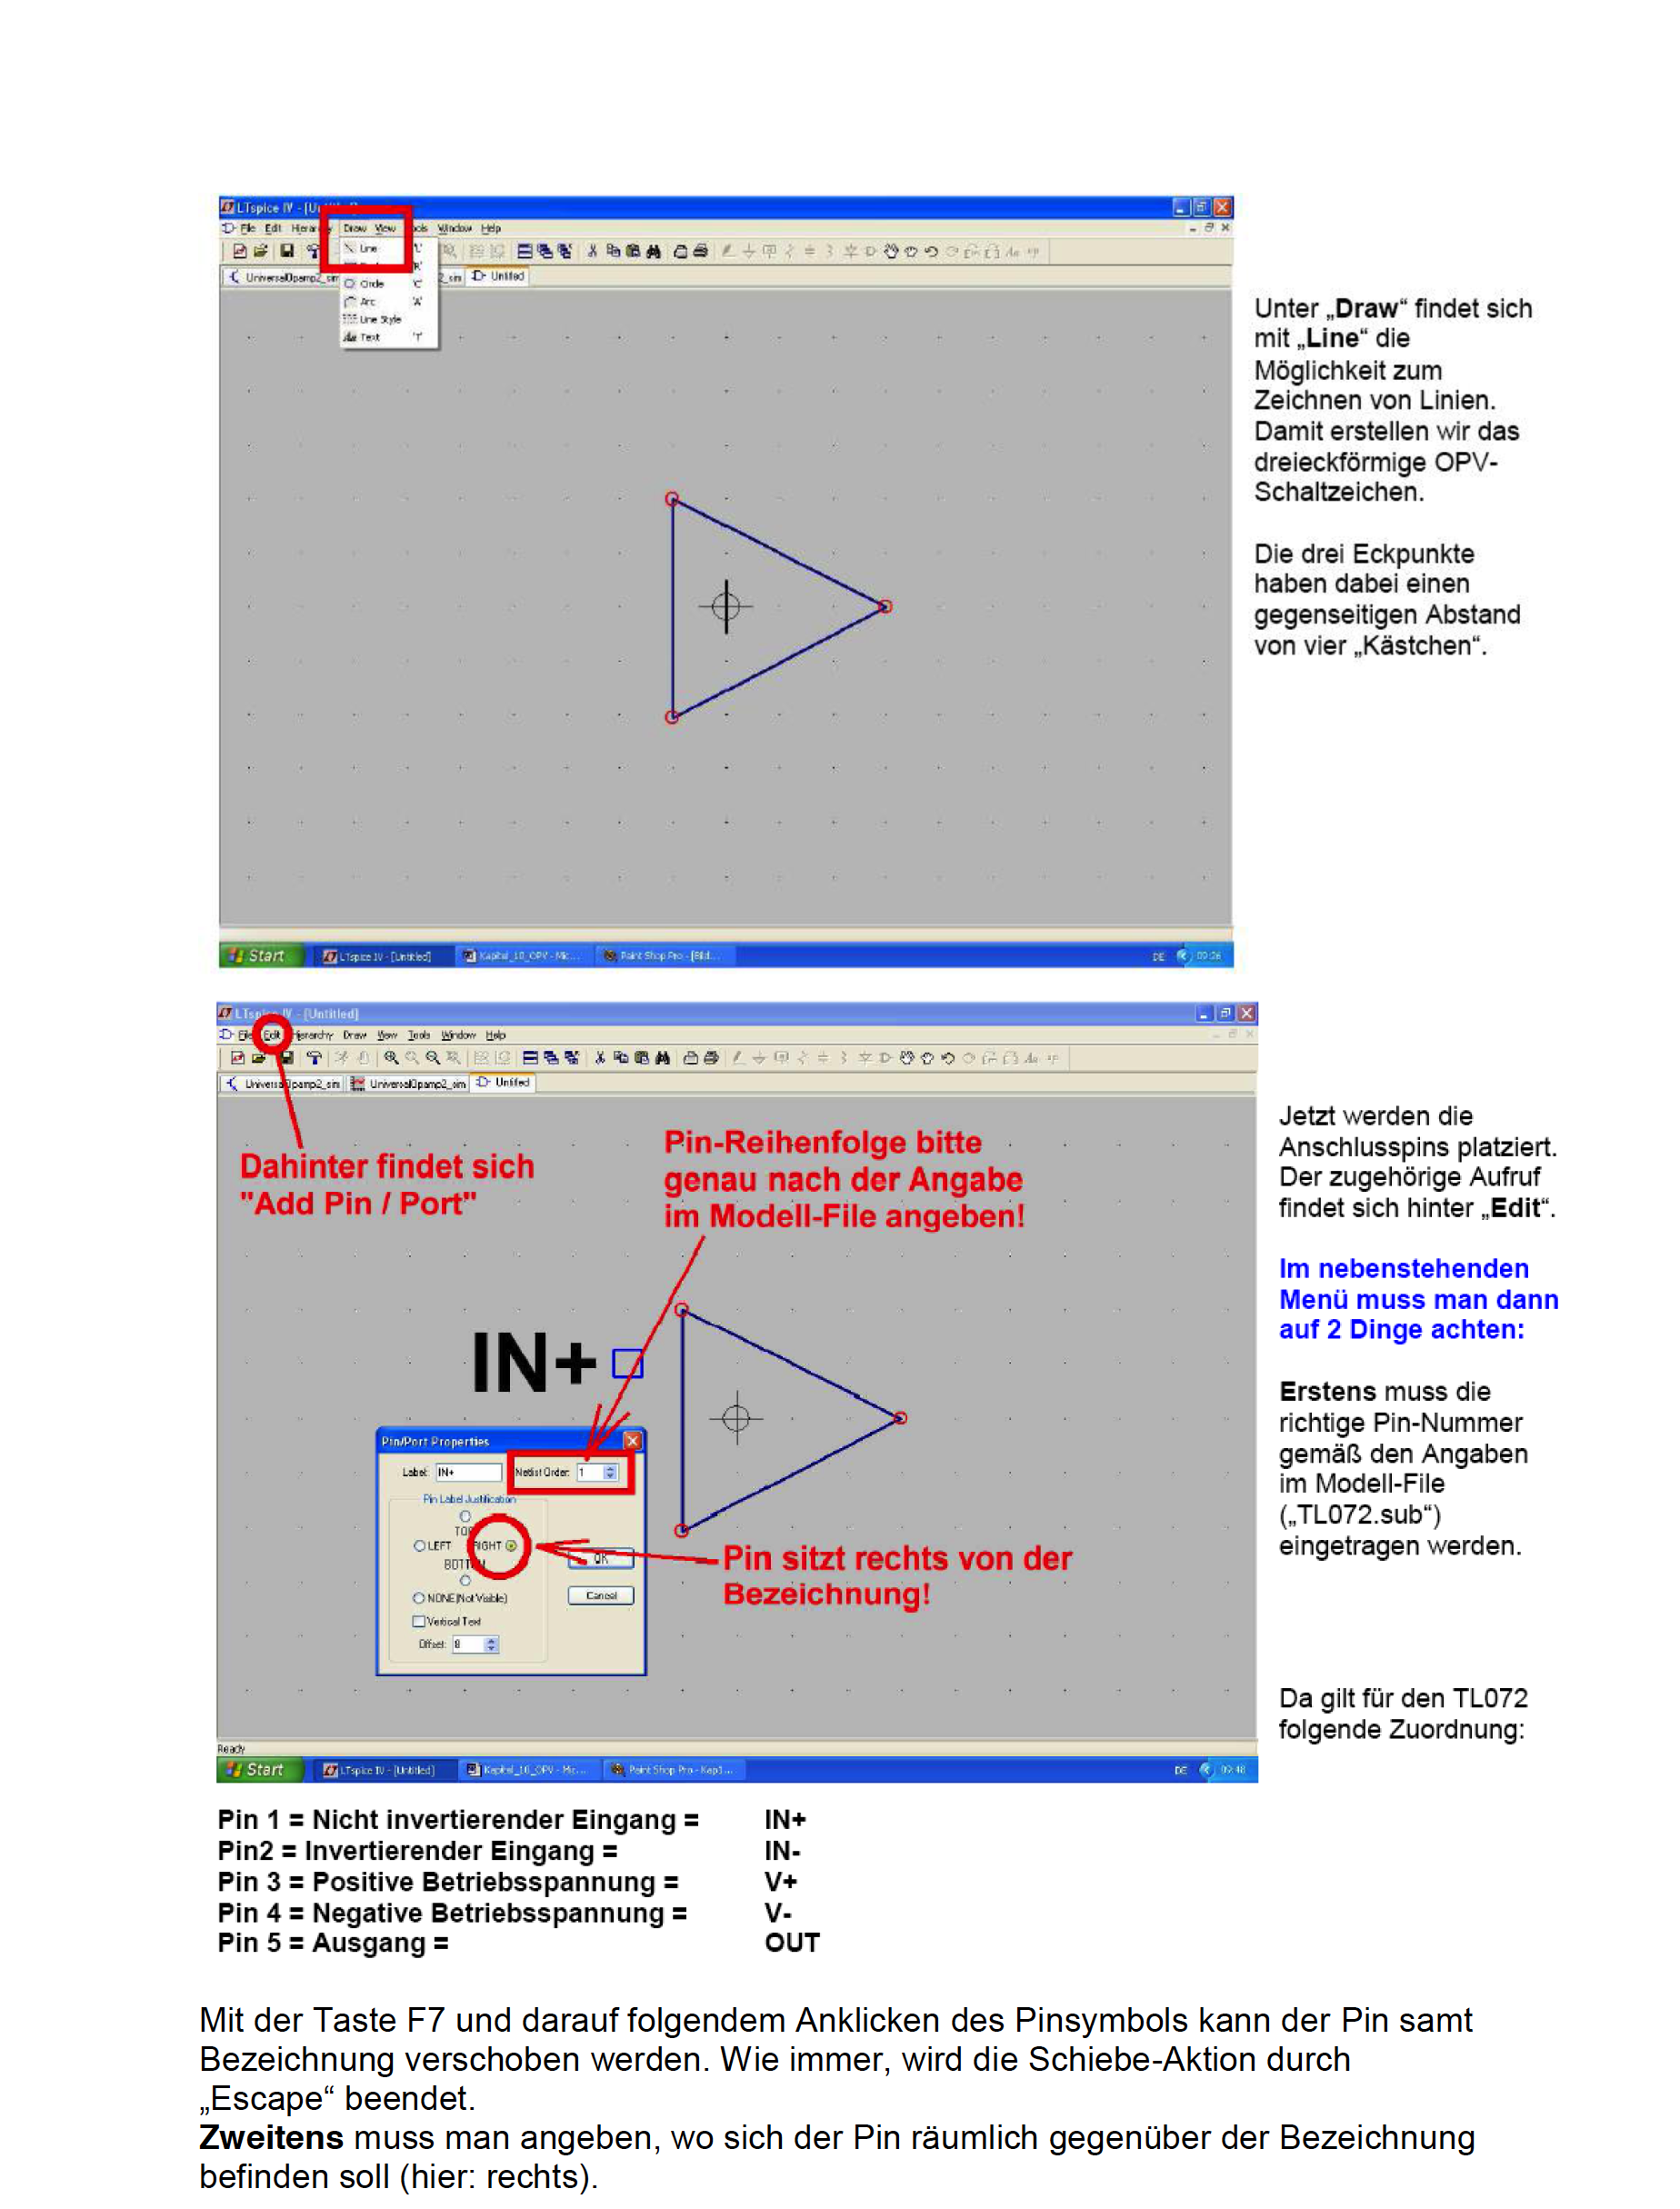
\includegraphics[width=\linewidth]{pictures/legacy/tl072_3.png}
            \end{minipage} 
            &
            \begin{minipage}{0.5\textwidth}
                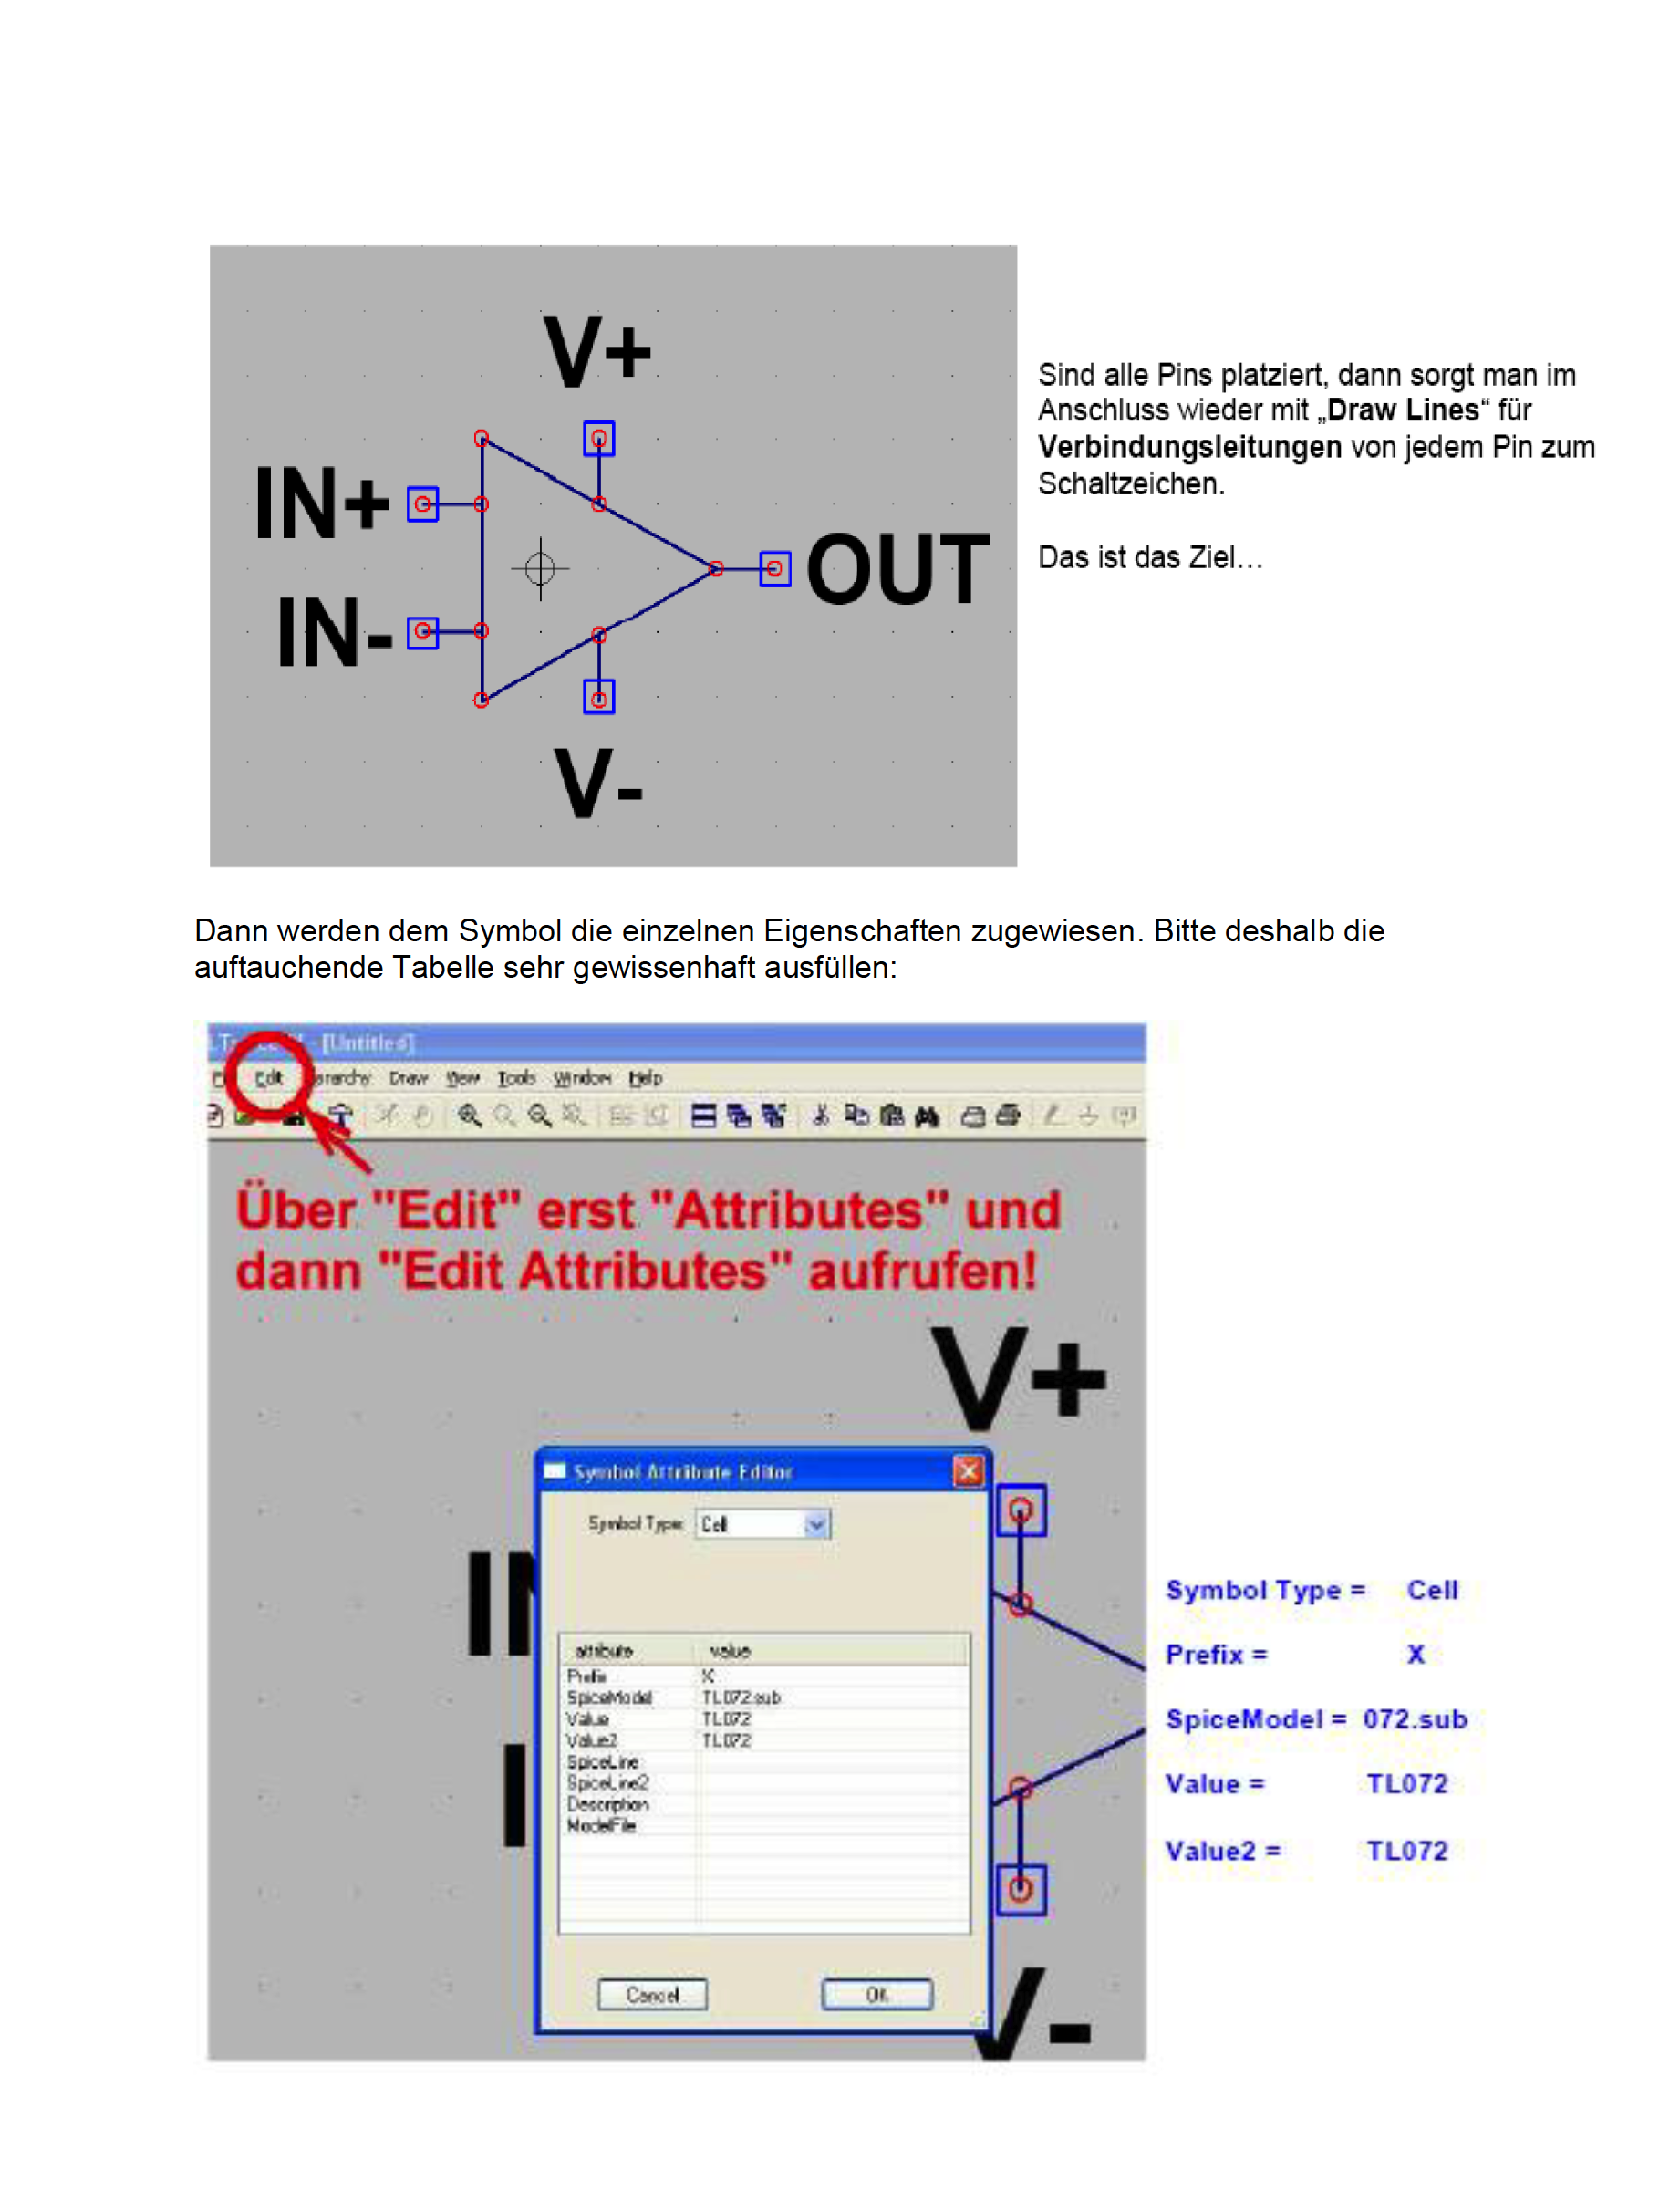
\includegraphics[width=\linewidth]{pictures/legacy/tl072_4.png}
            \end{minipage} 
      \end{tabular}
    \end{table}
    \end{tiny} \end{spacing}
\end{frame}

\begin{frame}[t]{Reale Bauteile modellieren mit einem subcircuit} 
    
    \begin{spacing}{0.9} \begin{tiny}
      \begin{table}[h!]
        \begin{tabular}{p{5cm} p{5cm}}
            \begin{minipage}{0.5\textwidth}                
                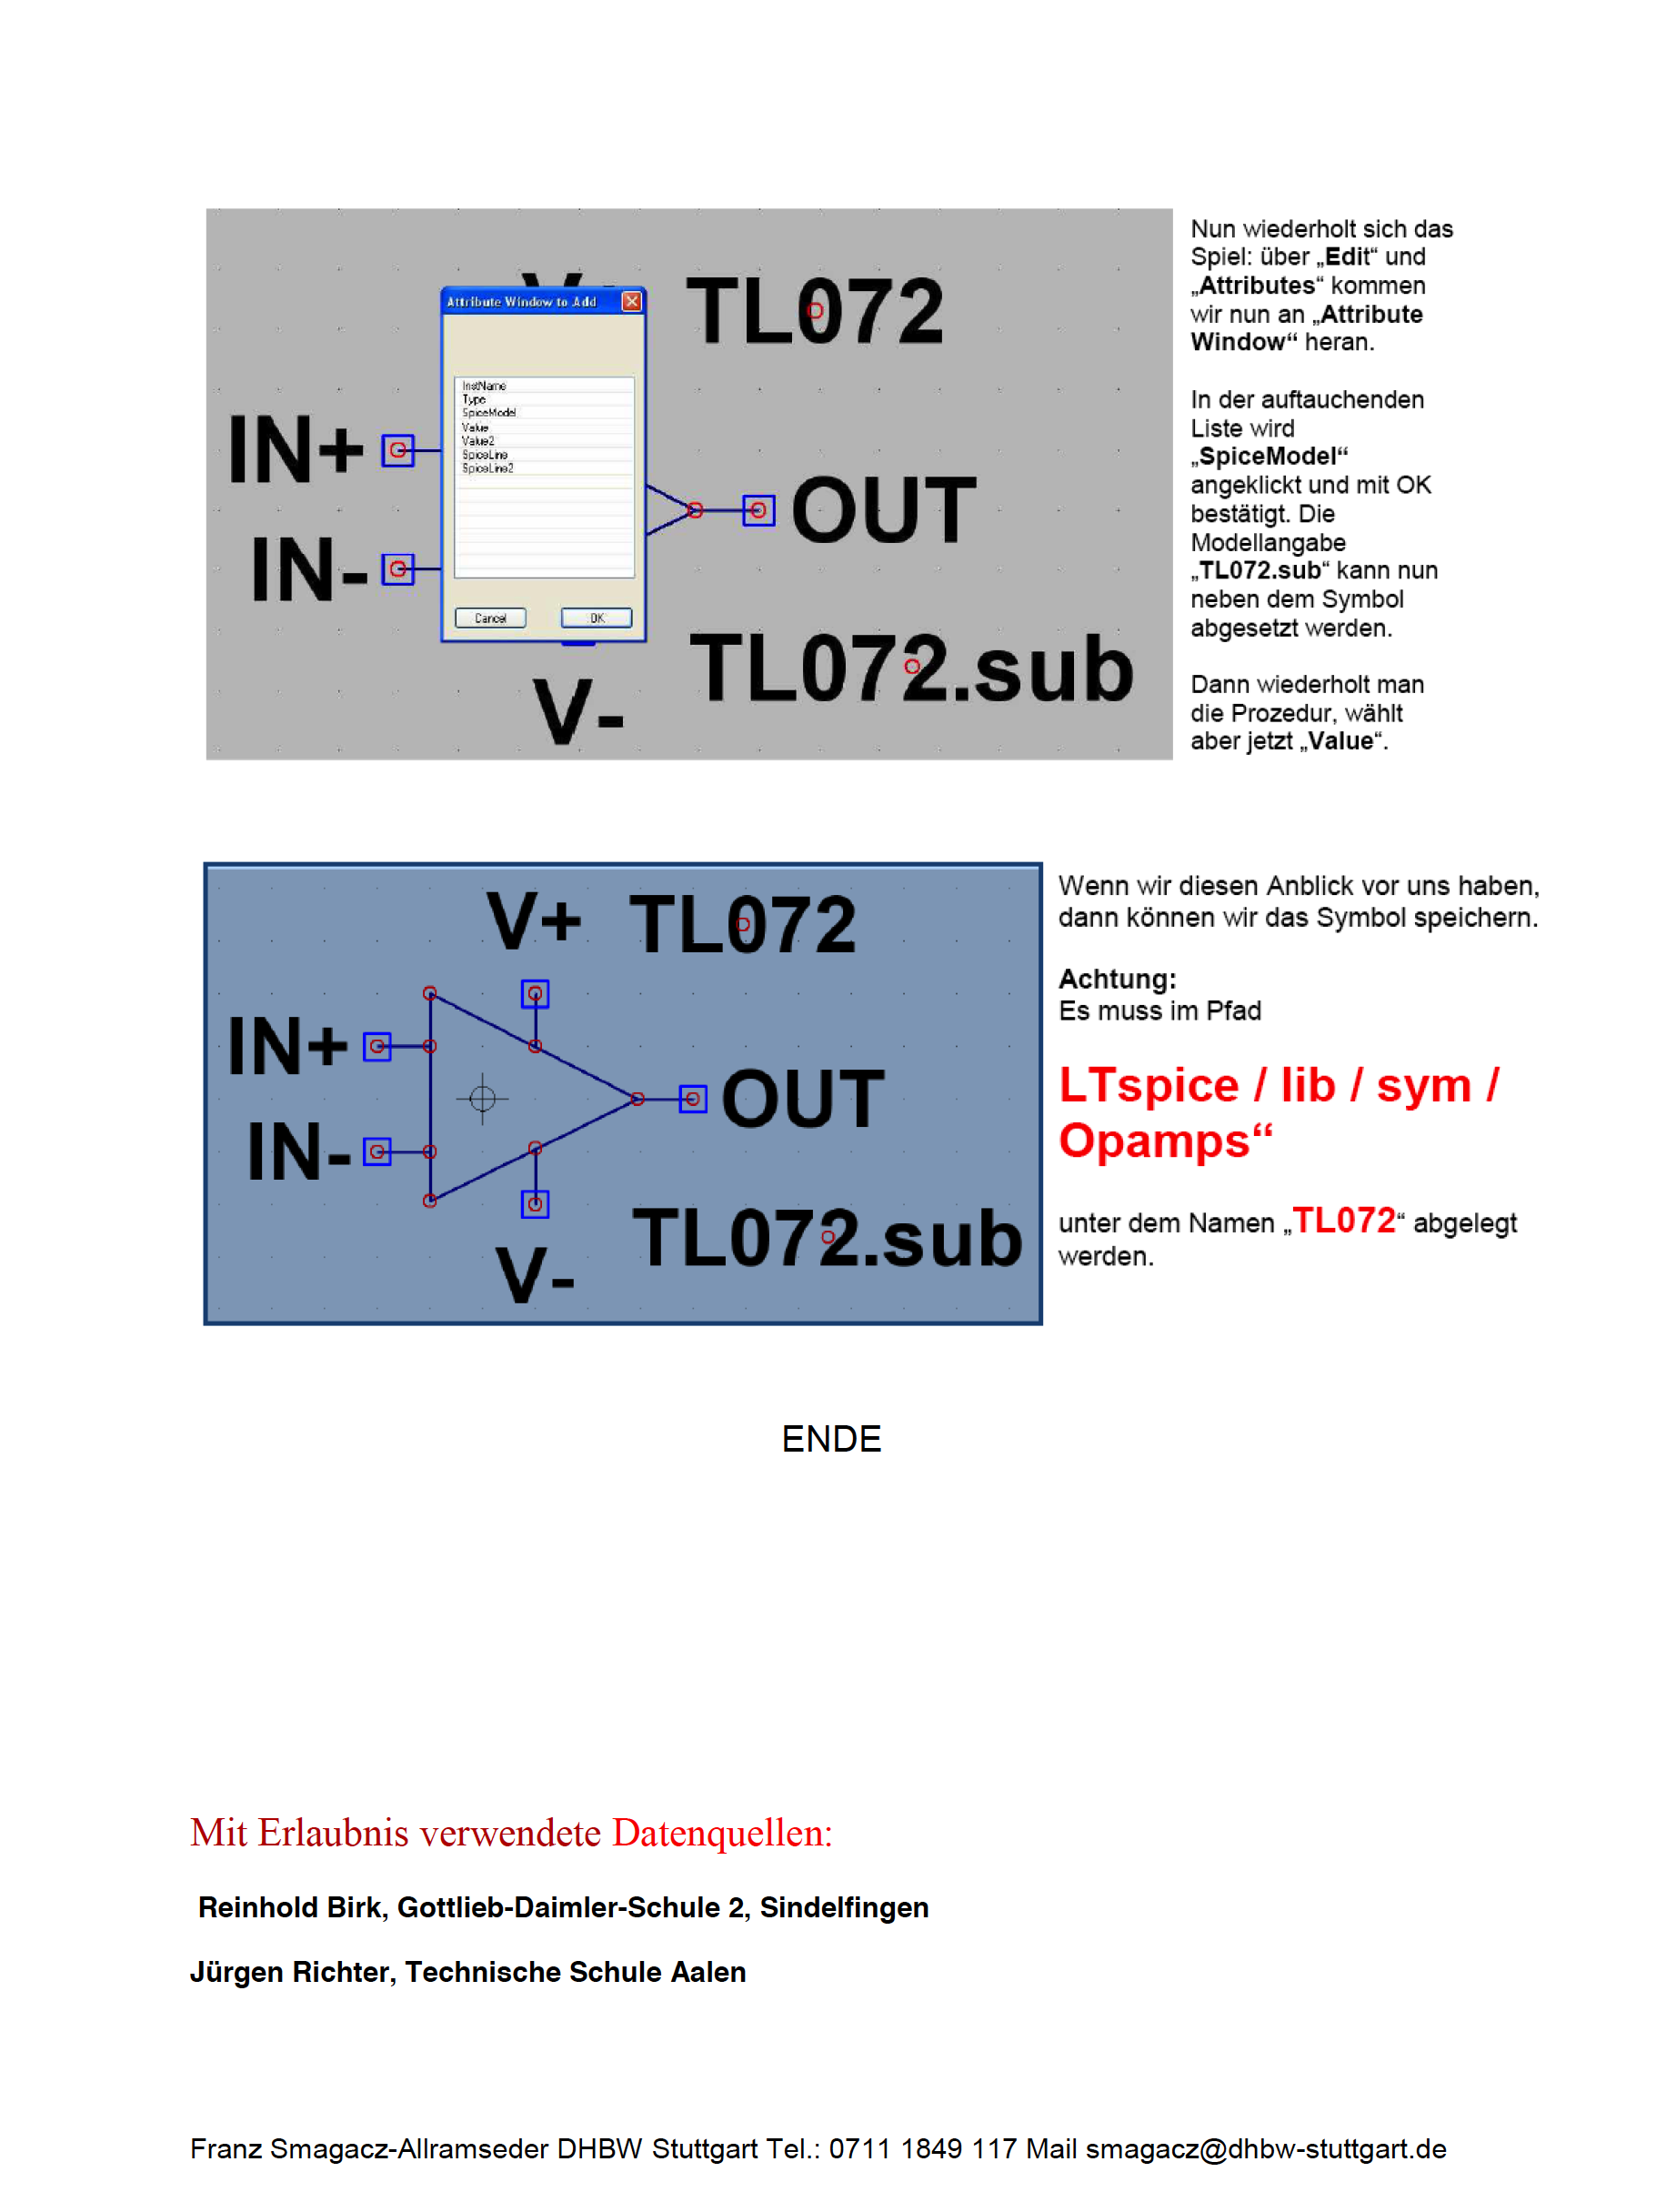
\includegraphics[width=\linewidth]{pictures/legacy/tl072_5.png}
            \end{minipage} 
            &
            \begin{minipage}{0.5\textwidth}
 
            \end{minipage} 
      \end{tabular}
    \end{table}
    \end{tiny} \end{spacing}
\end{frame}

\begin{frame}[t]{Digitale Schaltungssimulation} 
    
    \begin{spacing}{0.9} \begin{tiny}
      \begin{table}[h!]
        \begin{tabular}{p{5cm} p{5cm}}
            \begin{minipage}{0.5\textwidth}                
                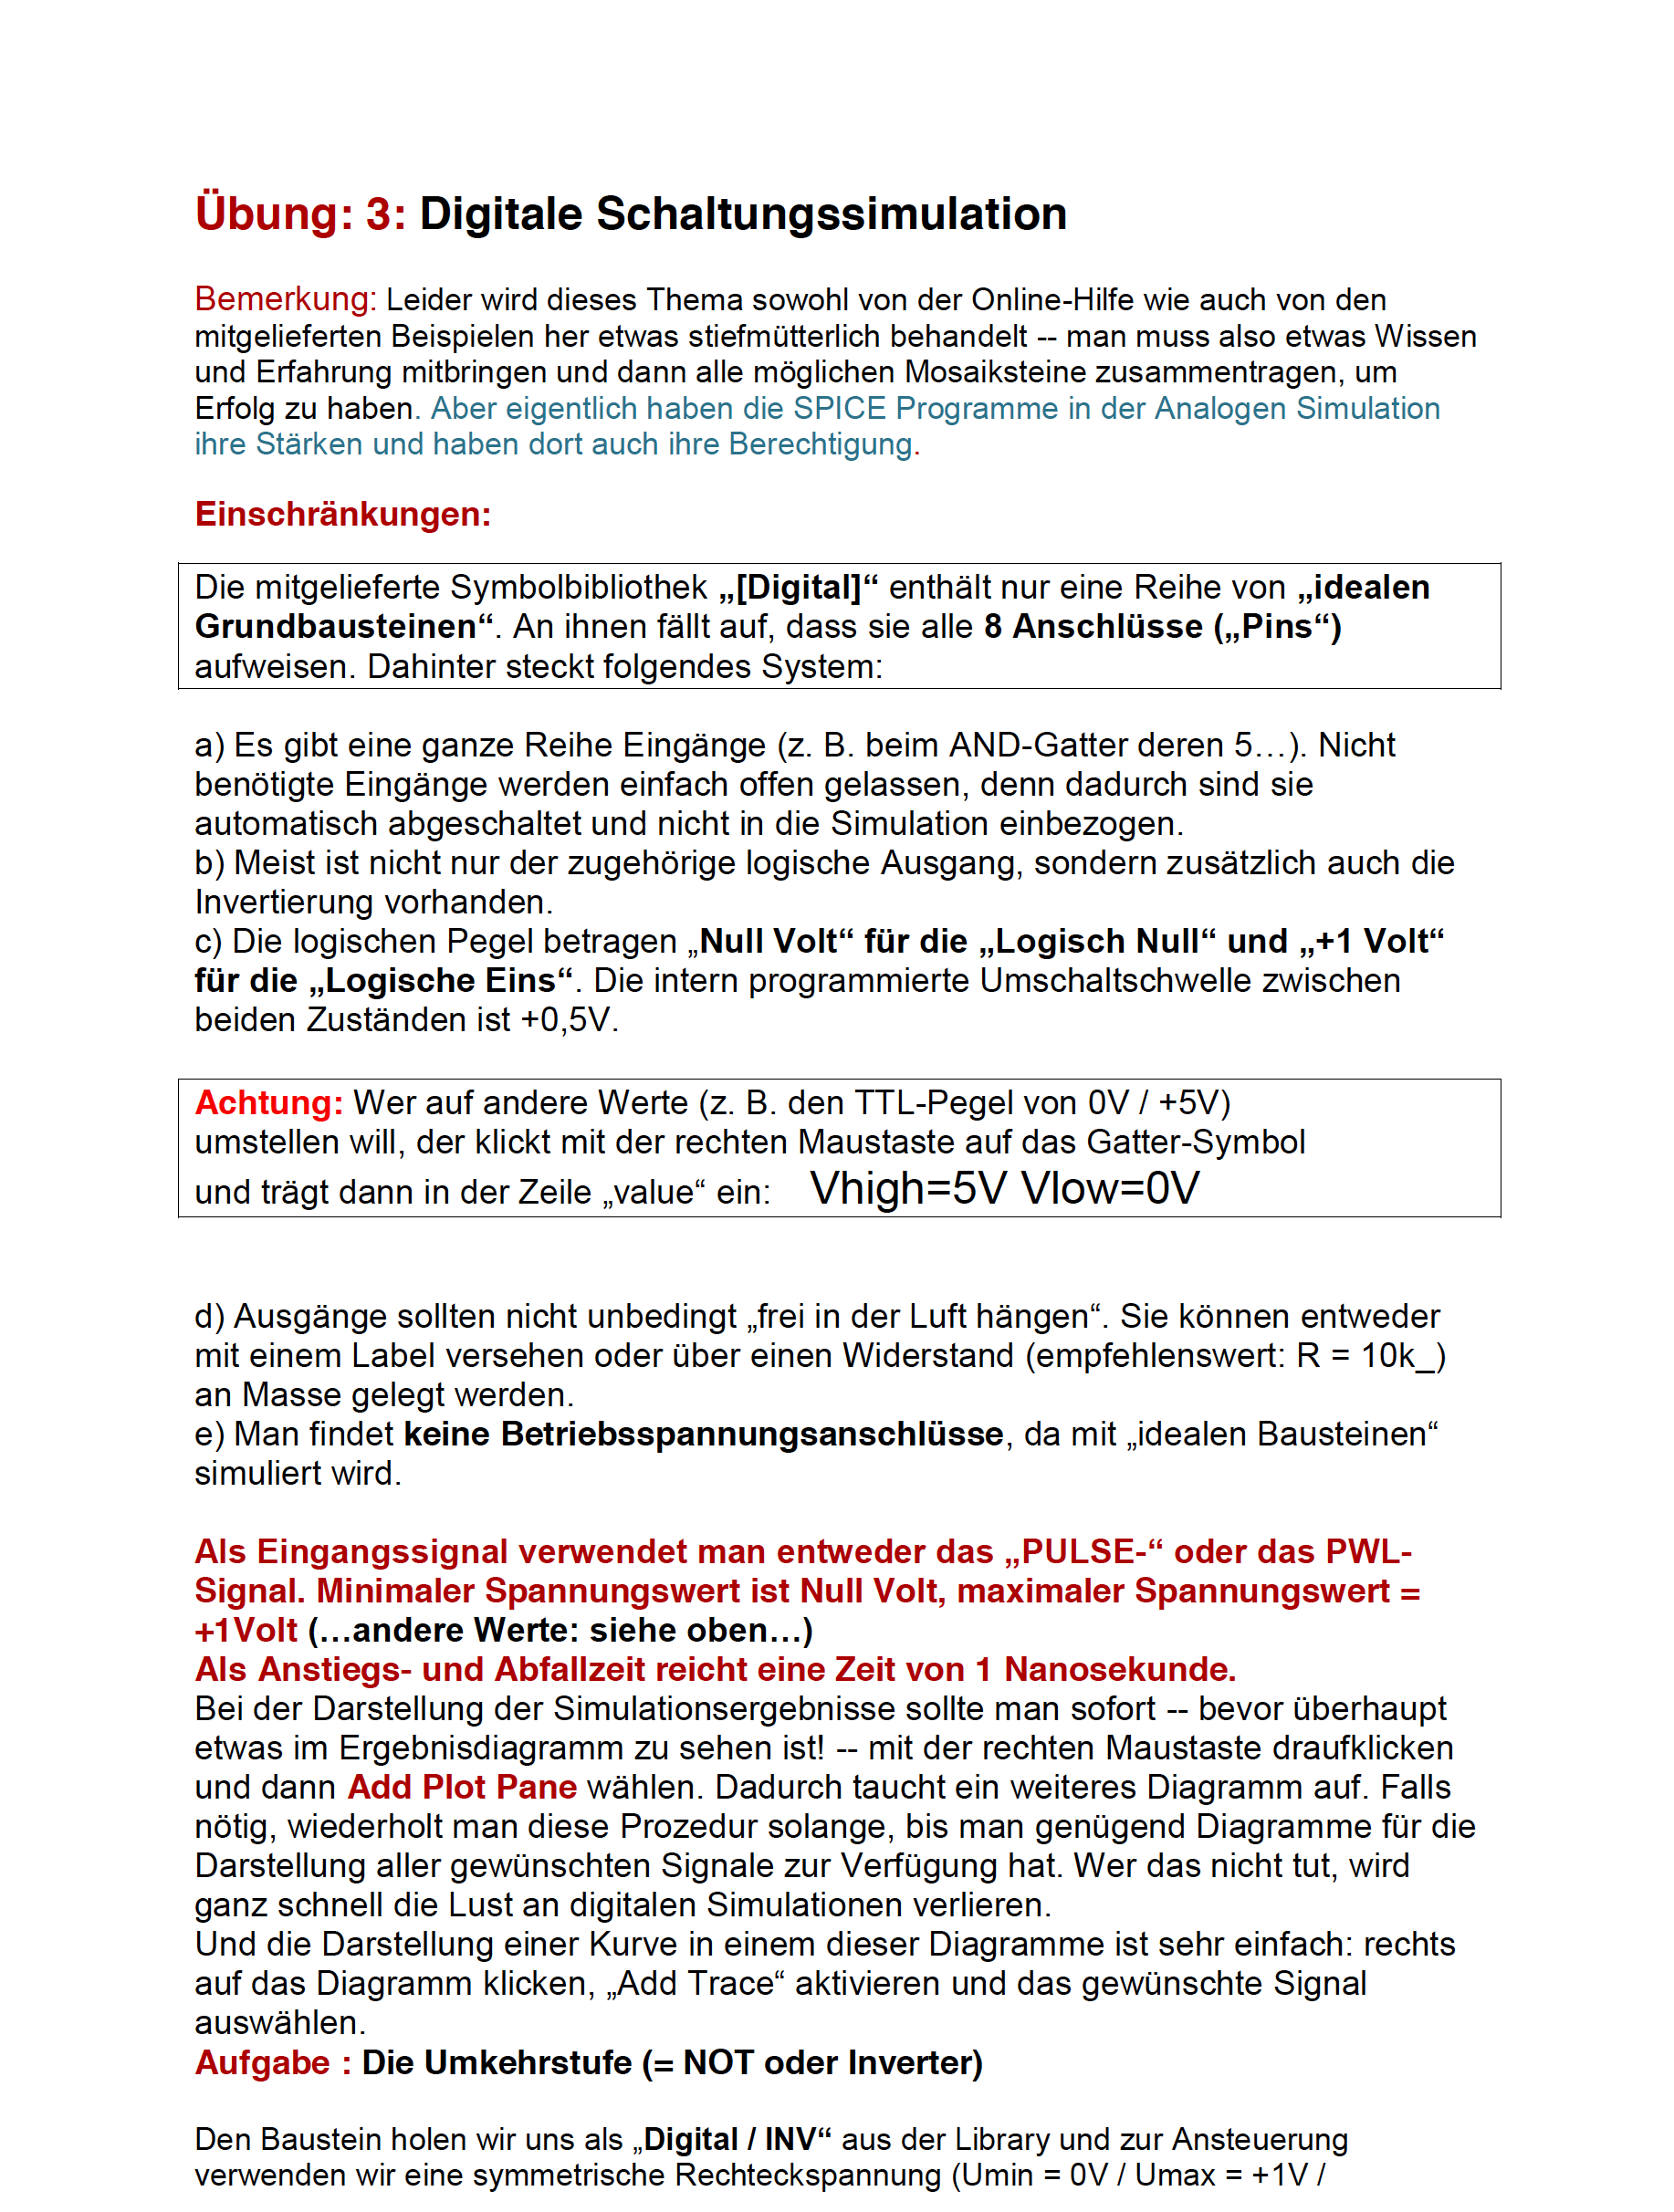
\includegraphics[width=\linewidth]{pictures/legacy/digi_1.png}
            \end{minipage} 
            &
            \begin{minipage}{0.5\textwidth}
                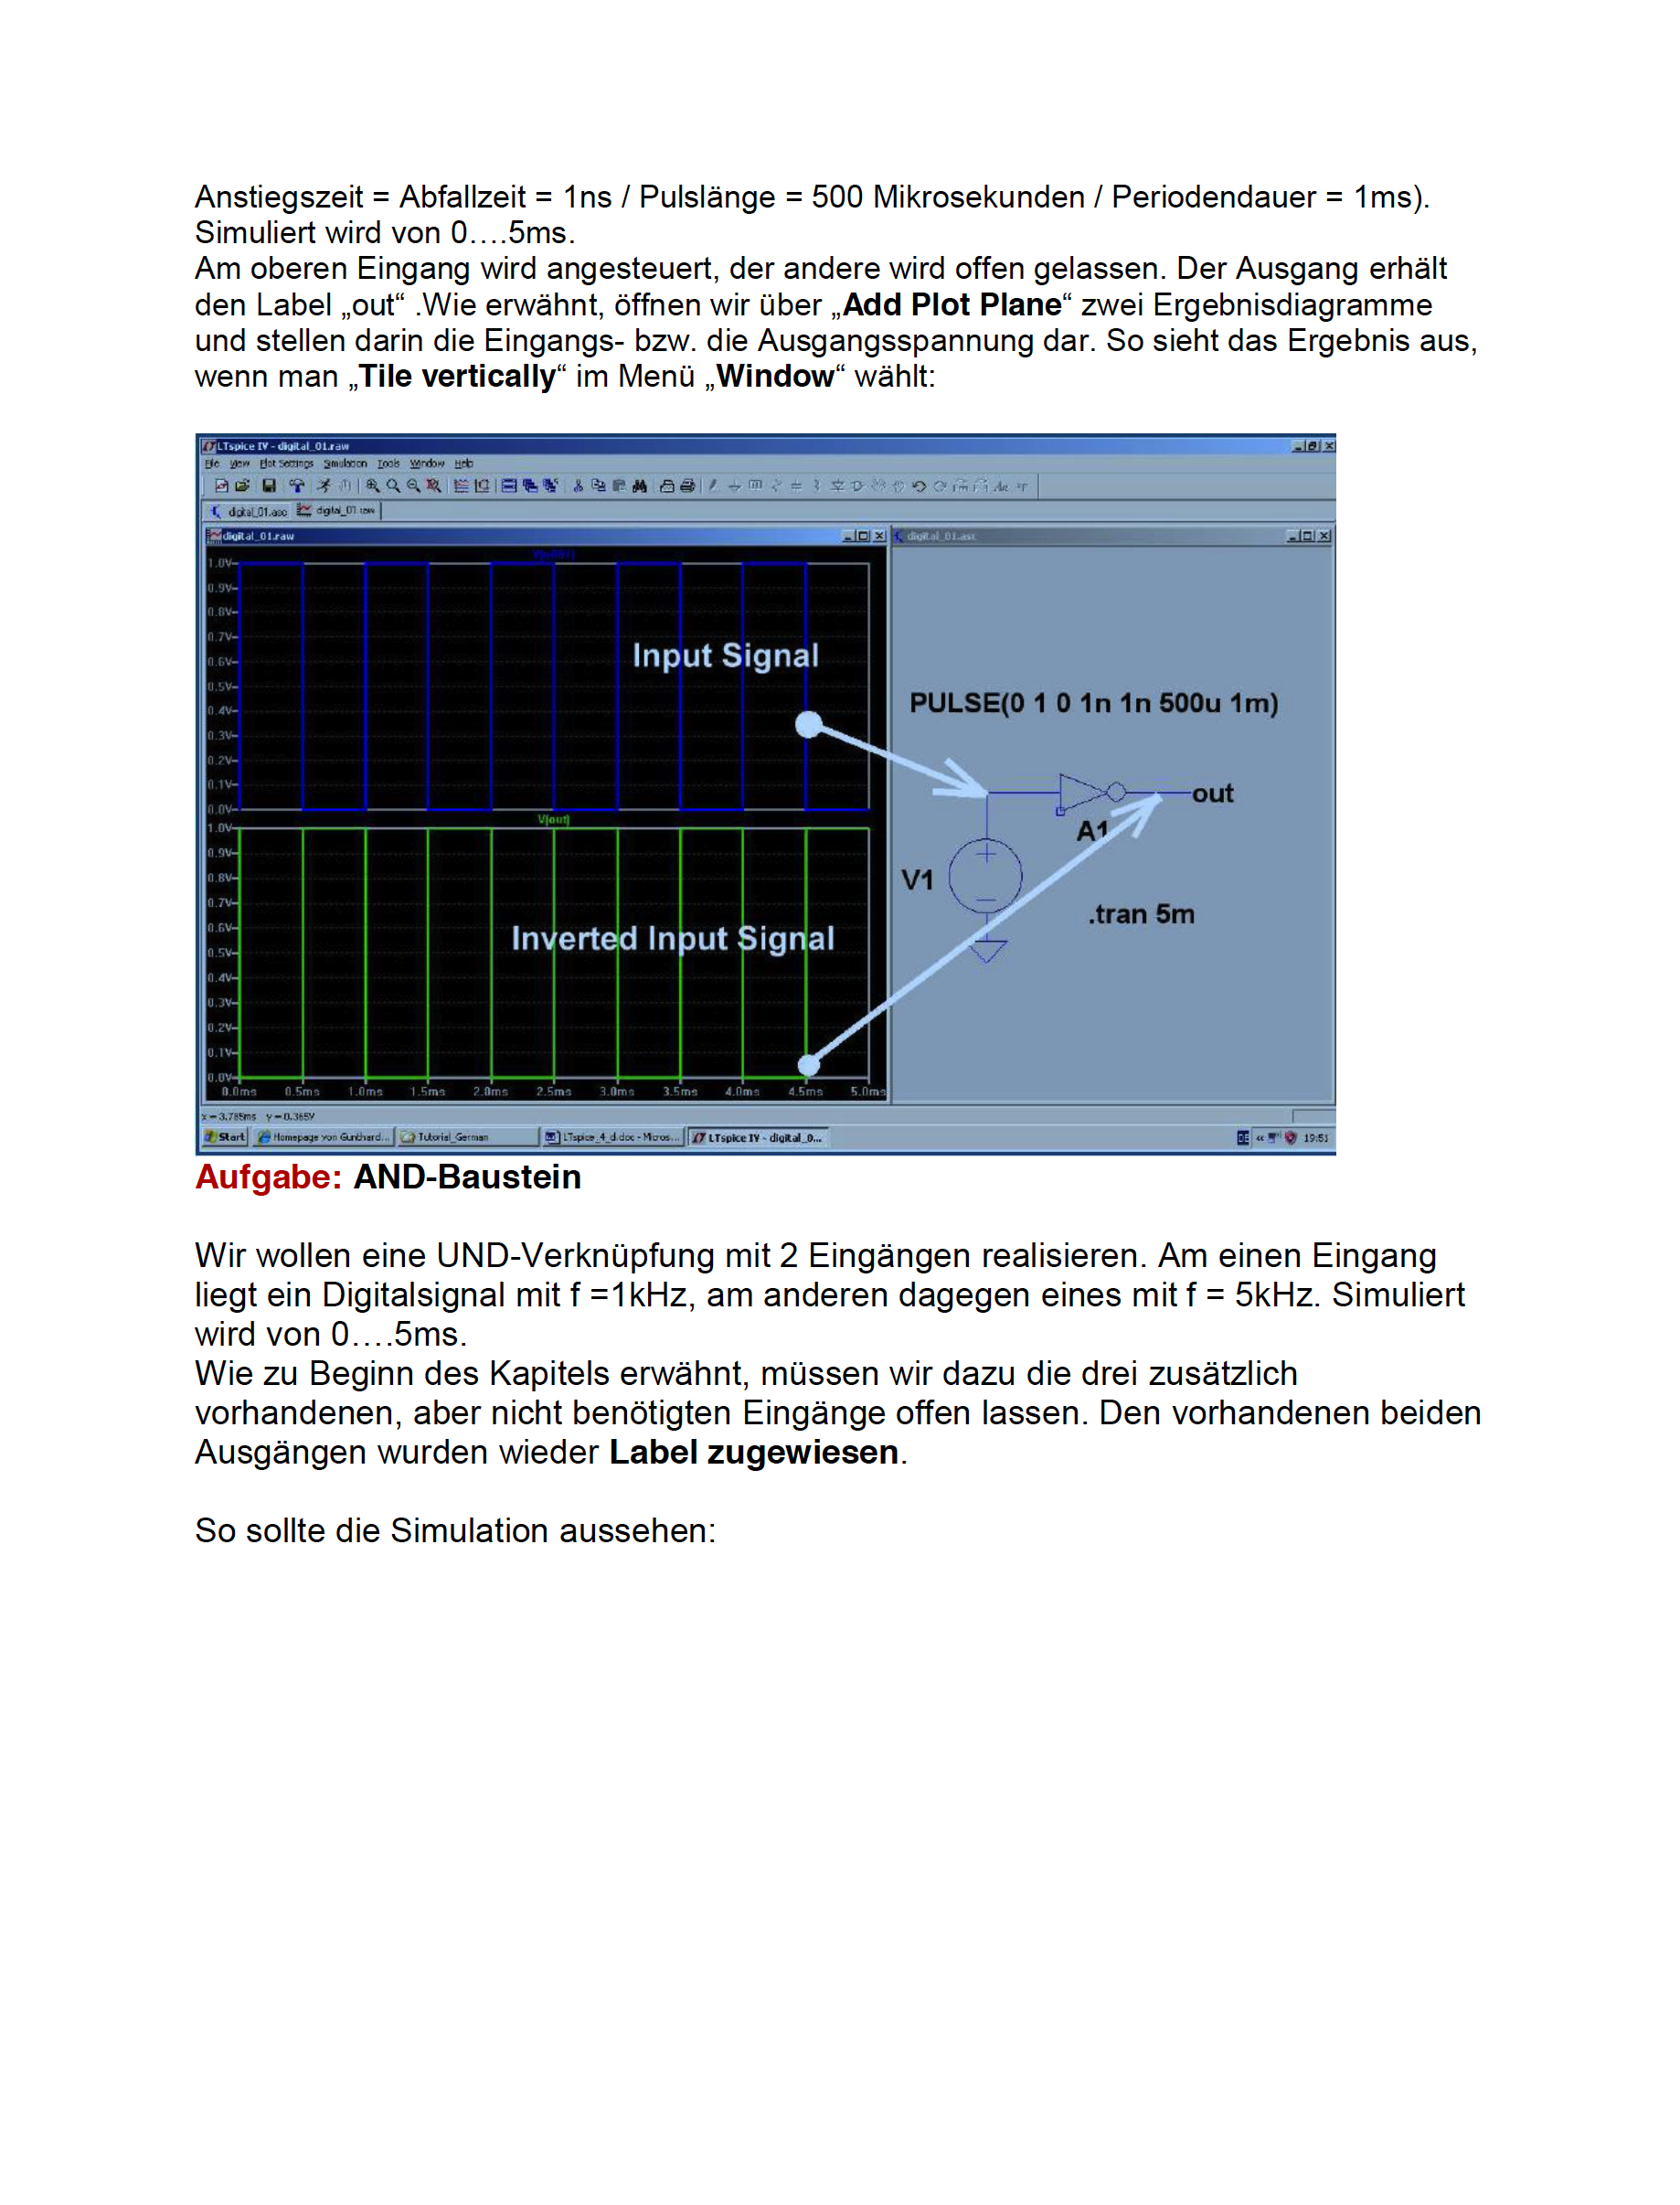
\includegraphics[width=\linewidth]{pictures/legacy/digi_2.png}
            \end{minipage} 
      \end{tabular}
    \end{table}
    \end{tiny} \end{spacing}
\end{frame}

\begin{frame}[t]{Reale Bauteile modellieren aus einem model file} 
    
    \begin{spacing}{0.9} \begin{tiny}
      \begin{table}[h!]
        \begin{tabular}{p{5cm} p{5cm}}
            \begin{minipage}{0.5\textwidth}                
                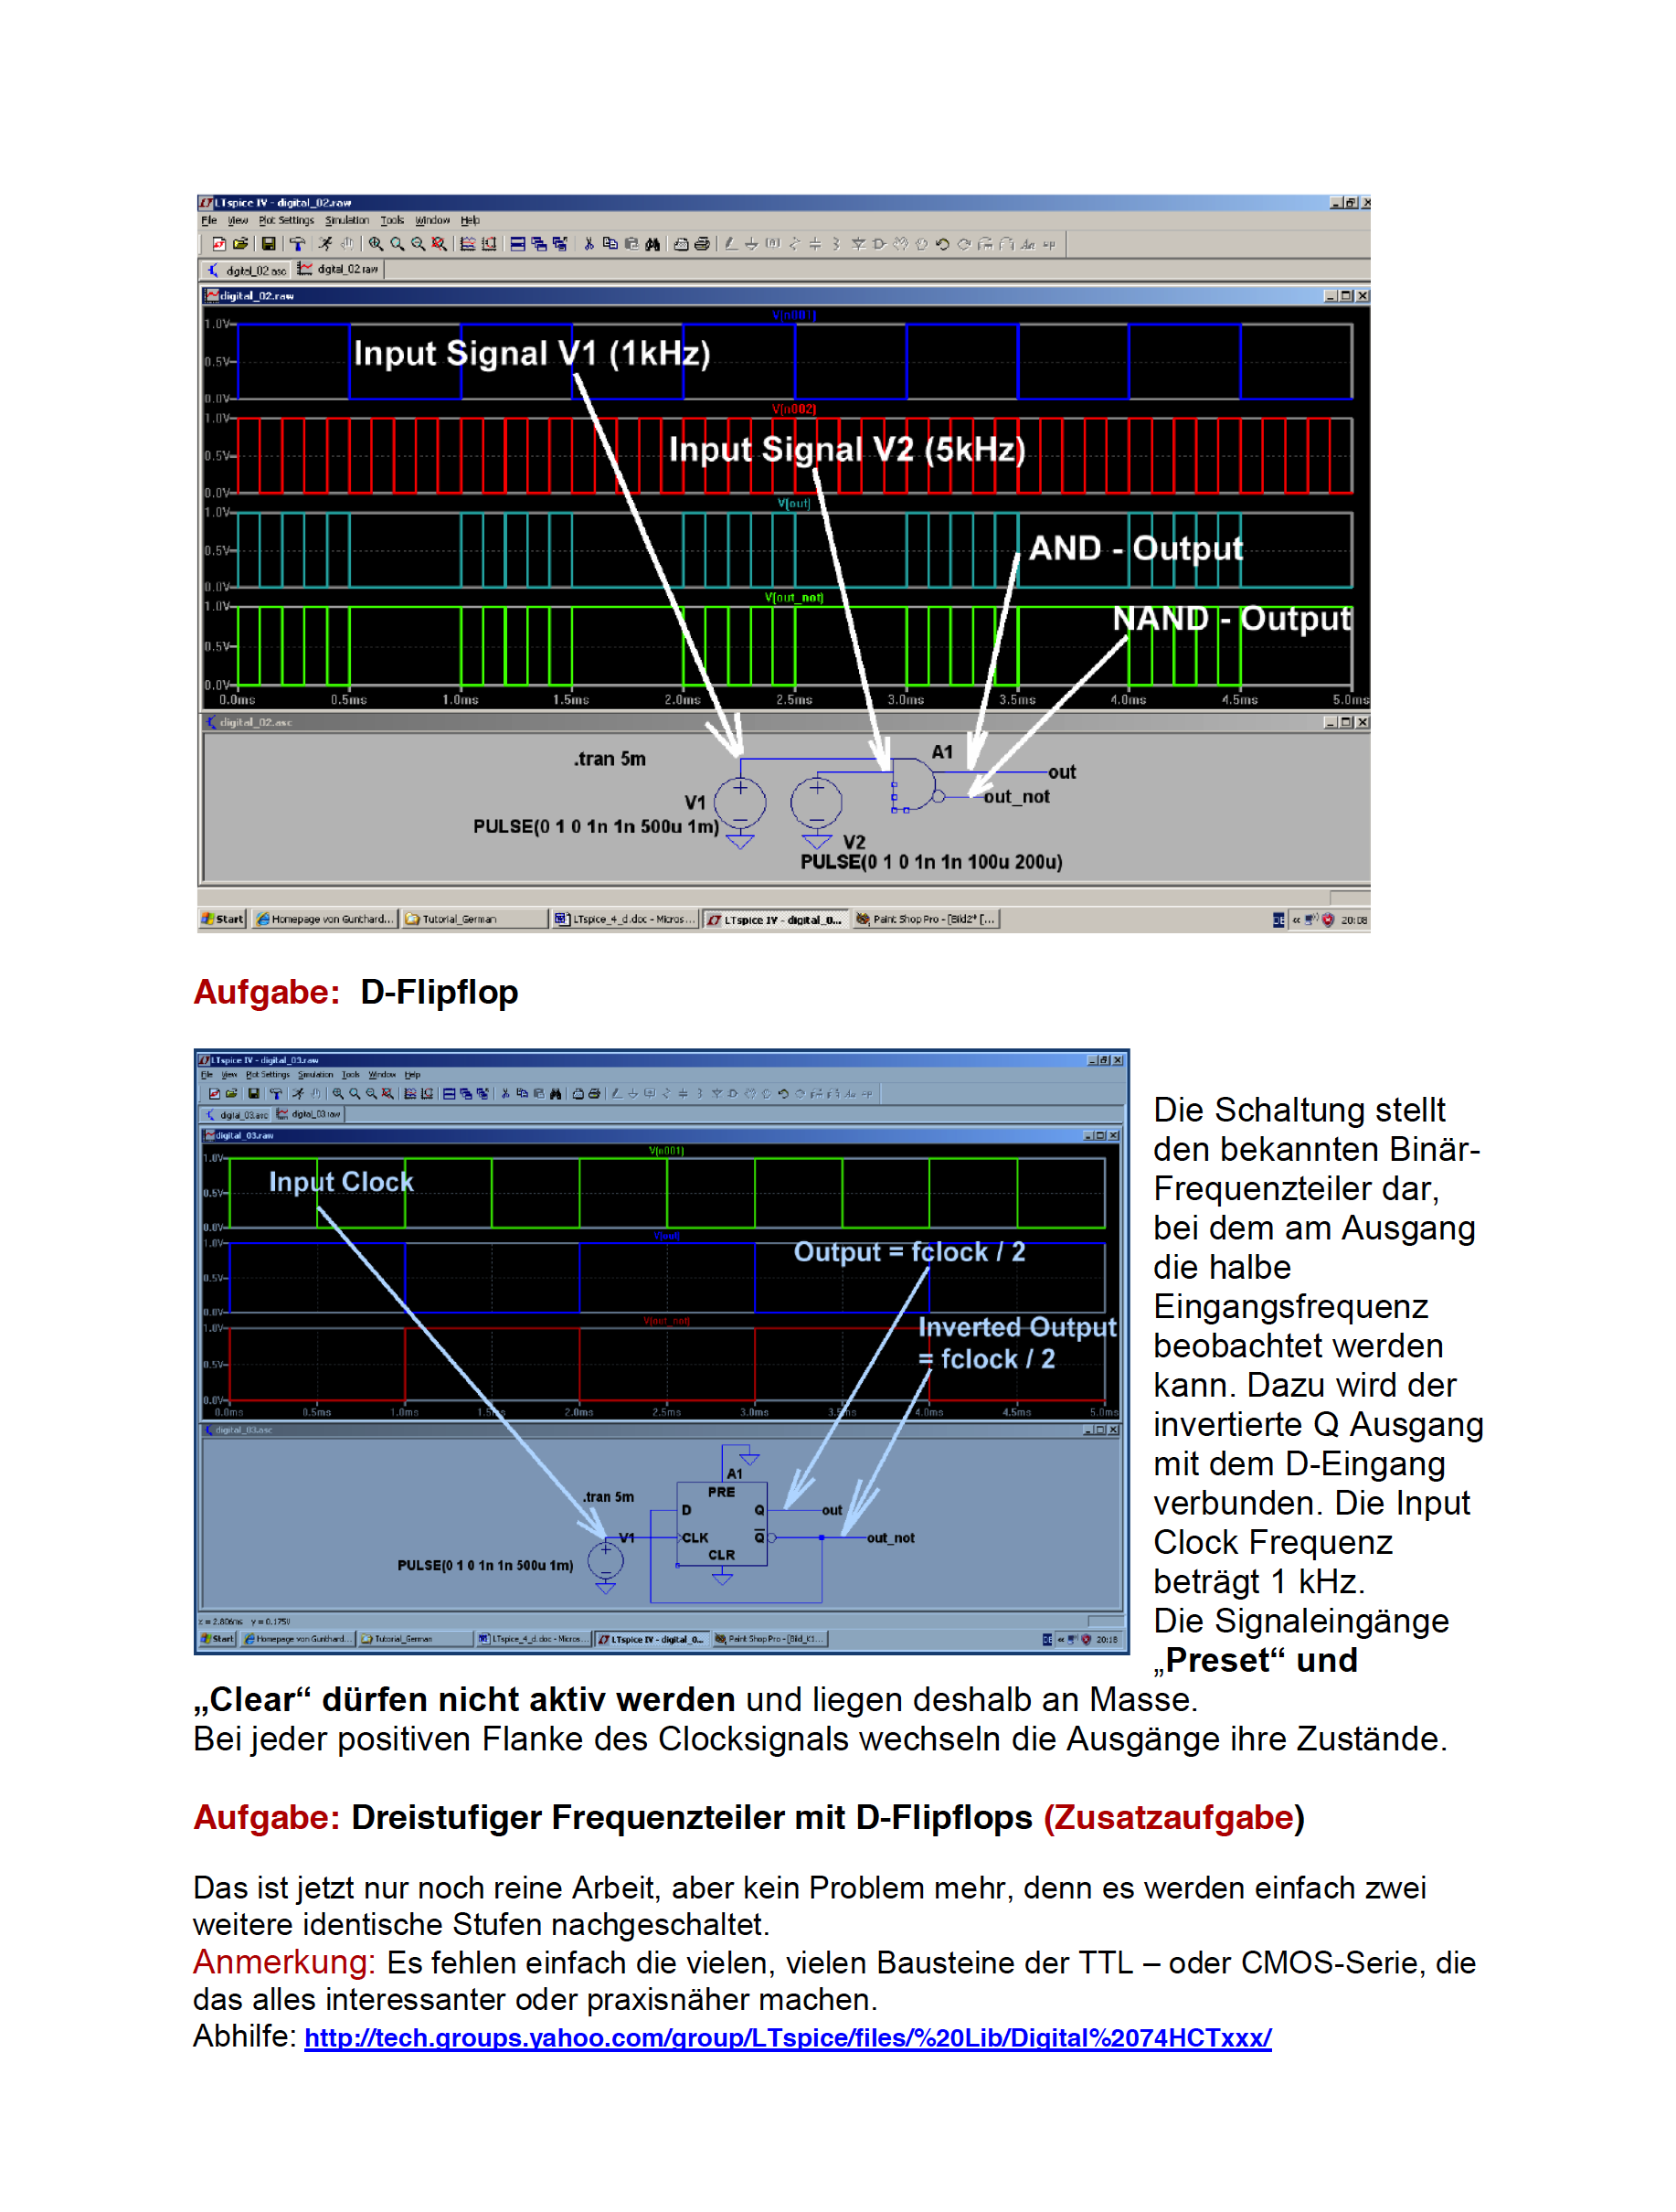
\includegraphics[width=\linewidth]{pictures/legacy/digi_3.png}
            \end{minipage} 
            &
            \begin{minipage}{0.5\textwidth}
                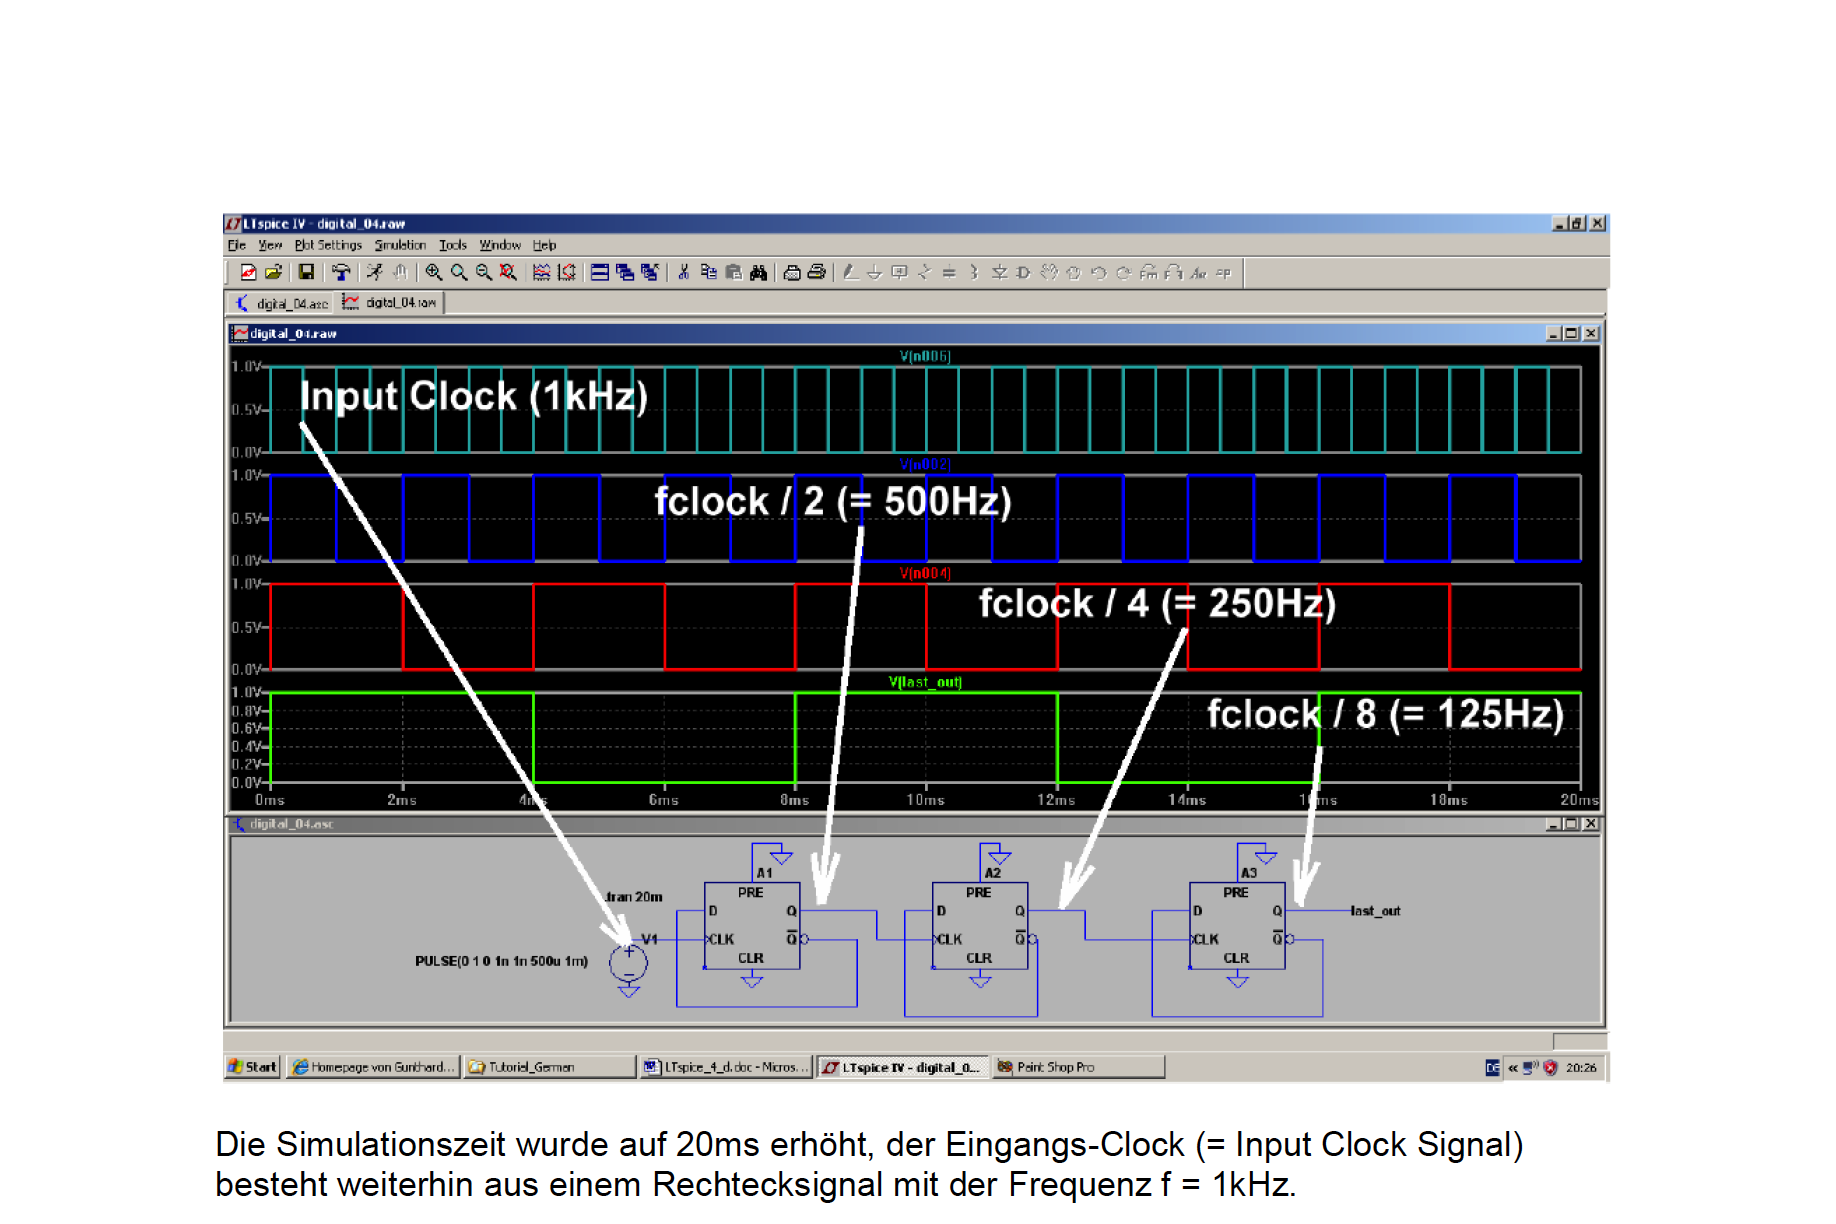
\includegraphics[width=\linewidth]{pictures/legacy/digi_4.png}
            \end{minipage} 
      \end{tabular}
    \end{table}
    \end{tiny} \end{spacing}
\end{frame}